\section{Hermite Algorithm for Periodicity Detection (\HAPD)}\label{sec:hapd_algorithm}

We present the Hermite-Algebraic Projective Descent (HAPD) algorithm, which characterizes cubic irrationals through eventual periodicity in three-dimensional projective space.

\subsection{Geometric Foundation}

\begin{definition}[Projective Space $\mathbb{P}^2(\mathbb{R})$]
The real projective plane $\mathbb{P}^2(\mathbb{R})$ is the set of equivalence classes of non-zero vectors $(v_1, v_2, v_3) \in \mathbb{R}^3 \setminus \{(0,0,0)\}$ under the equivalence relation $(v_1, v_2, v_3) \sim (tv_1, tv_2, tv_3)$ for any $t \in \mathbb{R} \setminus \{0\}$.
\end{definition}

\begin{definition}[Dirichlet Group $\Gamma_k$]\label{def:dirichlet_group}
Let $k$ be a cubic number field over $\mathbb{Q}$. The Dirichlet group $\Gamma_k$ is constructed as follows:

1. Let $\mathcal{O}_k$ be the ring of integers of $k$ and $\mathcal{O}_k^\times$ its unit group.

2. For a fixed basis $\{1, \alpha, \alpha^2\}$ of $k$ over $\mathbb{Q}$, where $\alpha$ is a primitive element, define the embedding:
\begin{equation}
\rho: k \to \text{GL}(3, \mathbb{R})
\end{equation}
by mapping each element to its matrix representation with respect to this basis.

3. The Dirichlet group $\Gamma_k$ is defined as:
\begin{equation}
\Gamma_k = \rho(\mathcal{O}_k^\times) \subset \text{GL}(3, \mathbb{R})
\end{equation}

This construction gives $\Gamma_k$ the structure of a discrete subgroup of $\text{GL}(3, \mathbb{R})$ that acts on $\mathbb{P}^2(\mathbb{R})$ via the standard projective action.
\end{definition}

\begin{lemma}[Properties of $\Gamma_k$]\label{lem:gamma_properties}
For a cubic field $k$, the Dirichlet group $\Gamma_k$ satisfies:
\begin{enumerate}
    \item It is a discrete subgroup of $\text{GL}(3, \mathbb{R})$
    \item It is commensurable with a subgroup of $\text{SL}(3, \mathbb{Z})$
    \item Its action on $\mathbb{P}^2(\mathbb{R})$ is properly discontinuous
\end{enumerate}
\end{lemma}

\begin{proof}
1. Discreteness follows from the fact that $\mathcal{O}_k^\times$ is finitely generated by Dirichlet's unit theorem.

2. Let $\mathcal{O}$ be the order generated by $\{1, \alpha, \alpha^2\}$. Then $\rho(\mathcal{O}^\times)$ is a subgroup of $\text{GL}(3, \mathbb{Z})$. Since $[\mathcal{O}_k : \mathcal{O}]$ is finite, $\Gamma_k$ is commensurable with $\rho(\mathcal{O}^\times)$.

3. The proper discontinuity follows from discreteness and the fact that $\text{GL}(3, \mathbb{R})$ acts properly on $\mathbb{P}^2(\mathbb{R})$.
\end{proof}

\begin{theorem}[Finite-Volume Fundamental Domain]\label{thm:finite_volume}
For a cubic number field $k$, the action of the Dirichlet group $\Gamma_k$ on $\mathbb{P}^2(\mathbb{R})$ has a fundamental domain of finite volume. Moreover, if $D$ is the discriminant of $k$, the volume is bounded by $O(|D|^{1/2} \log|D|)$.
\end{theorem}

\begin{proof}
By Lemma \ref{lem:gamma_properties}, $\Gamma_k$ is a discrete subgroup of $\text{GL}(3, \mathbb{R})$ commensurable with a subgroup of $\text{SL}(3, \mathbb{Z})$. By Borel and Harish-Chandra's theorem on arithmetic groups \cite{BH62}, such groups have finite covolume.

For the explicit bound, we use:
1. The regulator $R_k$ of $k$ satisfies $R_k = O(\sqrt{|D|}\log|D|)$ by Landau's bound
2. The fundamental domain volume is proportional to $R_k$ by the construction of $\Gamma_k$
3. The action on $\mathbb{P}^2(\mathbb{R})$ preserves this volume bound
\end{proof}

\begin{remark}
The explicit calculation of the volume of the fundamental domain provides an effective bound on the number of iterations required for the HAPD algorithm to detect periodicity. For a cubic field with discriminant $D$, this bound is $O(|D|^{1/2} \log|D|)$, as established by Minkowski's geometry of numbers and refined by estimates on the regulator.
\end{remark}

\subsection{The HAPD Algorithm and its Relation to the Dirichlet Group}

The HAPD algorithm operates in the projective space $\mathbb{P}^2(\mathbb{R})$ and effectively detects the action of the Dirichlet group $\Gamma_k$ on this space.

\begin{theorem}[HAPD and Dirichlet Group Correspondence]\label{thm:hapd_dirichlet}
The HAPD transformation $T: (v_1, v_2, v_3) \mapsto (r_1, r_2, v_3 - a_1r_1 - a_2r_2)$ corresponds to an element of the Dirichlet group $\Gamma_k$ acting on $\mathbb{P}^2(\mathbb{R})$, where $k = \mathbb{Q}(v_1/v_3)$.
\end{theorem}

\begin{proof}
For a cubic irrational $\alpha = v_1/v_3$, the triplet $(v_1, v_2, v_3) = (v_3\alpha, v_3\alpha^2, v_3)$ represents a point in projective space.

The HAPD transformation computes:
\begin{align}
a_1 &= \lfloor v_1/v_3 \rfloor\\
a_2 &= \lfloor v_2/v_3 - a_1(v_1/v_3) \rfloor = \lfloor \alpha^2 - a_1\alpha \rfloor\\
r_1 &= v_1 - a_1v_3\\
r_2 &= v_2 - a_1v_1 - a_2v_3
\end{align}

This transformation can be represented by a matrix $M_T \in \text{GL}(3, \mathbb{R})$ acting on the vector $(v_1, v_2, v_3)^T$.

Let $\beta = \frac{1}{\alpha - a_1 - \frac{a_2}{\alpha}}$. Then $\beta \in \mathbb{Q}(\alpha)$ and represents a unit element in the cubic field. The matrix representation of multiplication by $\beta$ in the basis $\{1, \alpha, \alpha^2\}$ corresponds precisely to the HAPD transformation after projective normalization.

Thus, the HAPD transformation $T$ corresponds to the action of an element of the Dirichlet group $\Gamma_k$ on $\mathbb{P}^2(\mathbb{R})$.
\end{proof}

\begin{theorem}[Periodicity via Dirichlet's Pigeonhole]\label{thm:periodicity}
The HAPD algorithm produces an eventually periodic sequence for cubic irrationals.
\end{theorem}

\begin{proof}
For a cubic irrational $\alpha$, the HAPD algorithm produces a sequence of points $(v_1^{(n)}, v_2^{(n)}, v_3^{(n)})$ in $\mathbb{P}^2(\mathbb{R})$.

By Theorem \ref{thm:hapd_dirichlet}, each step corresponds to the action of an element of the Dirichlet group $\Gamma_k$. The sequence of points remains within the cubic field $k = \mathbb{Q}(\alpha)$.

From Theorem \ref{thm:finite_volume}, the action of $\Gamma_k$ on $\mathbb{P}^2(\mathbb{R})$ has a fundamental domain of finite volume. The sequence of points must eventually enter the same fundamental domain translation, implying that there exist indices $m < n$ such that:
\begin{equation}
(v_1^{(n)}, v_2^{(n)}, v_3^{(n)}) = \gamma \cdot (v_1^{(m)}, v_2^{(m)}, v_3^{(m)})
\end{equation}
for some $\gamma \in \Gamma_k$.

Since the HAPD transformation is deterministic, this implies that the sequence is eventually periodic with period dividing $n-m$.

An explicit upper bound on the period length can be derived from the effective volume estimate given in the remark after Theorem \ref{thm:finite_volume}.
\end{proof}

\subsection{Algorithm Description}

The HAPD algorithm operates on triples $(v_1, v_2, v_3)$ representing points in $\mathbb{P}^2(\mathbb{R})$.

\begin{algorithm}[H]
\caption{Hermite-Algebraic Projective Descent (HAPD) Algorithm}
\label{alg:hapd}
\begin{algorithmic}[1]
\Require Real number $\alpha$ to be tested for being a cubic irrational
\State Initialize $(v_1, v_2, v_3) \gets (\alpha, \alpha^2, 1)$
\State $S \gets \emptyset$ \Comment{Set to store visited states}
\While{$(v_1, v_2, v_3) \not\in S$}
    \State Add normalized $(v_1, v_2, v_3)$ to $S$
    \State $a_1 \gets \lfloor v_1/v_3 \rfloor$
    \State $a_2 \gets \lfloor (v_2 - a_1v_1)/v_3 \rfloor$
    \State $r_1 \gets v_1 - a_1v_3$
    \State $r_2 \gets v_2 - a_1v_1 - a_2v_3$
    \State $(v_1, v_2, v_3) \gets (r_1, r_2, v_3 - a_1r_1 - a_2r_2)$
\EndWhile
\State \Return "Cubic irrational" and the period
\end{algorithmic}
\end{algorithm}

\begin{theorem}[Cubic Characterization]\label{thm:cubic_periodic}
If $\alpha$ is a cubic irrational, then the HAPD algorithm produces an eventually periodic sequence.
\end{theorem}

\begin{proof}
This follows directly from Theorem \ref{thm:periodicity}.
\end{proof}

\begin{theorem}[Only Cubic Periodicity]\label{thm:only_cubic_periodic}
If the HAPD algorithm produces an eventually periodic sequence for input $\alpha$, then $\alpha$ is a cubic irrational.
\end{theorem}

\begin{proof}
If $\alpha$ is rational or quadratic irrational, the HAPD sequence either terminates or enters a subspace of dimension less than 3.

For non-algebraic or higher-degree algebraic numbers, the orbit under the action of the Dirichlet group does not remain in a discrete set, and by the ergodicity of the action on $\mathbb{P}^2(\mathbb{R})$, the sequence cannot be periodic.

Therefore, periodicity in the HAPD algorithm characterizes exactly the cubic irrationals.
\end{proof}

\begin{figure}[htbp]
\centering
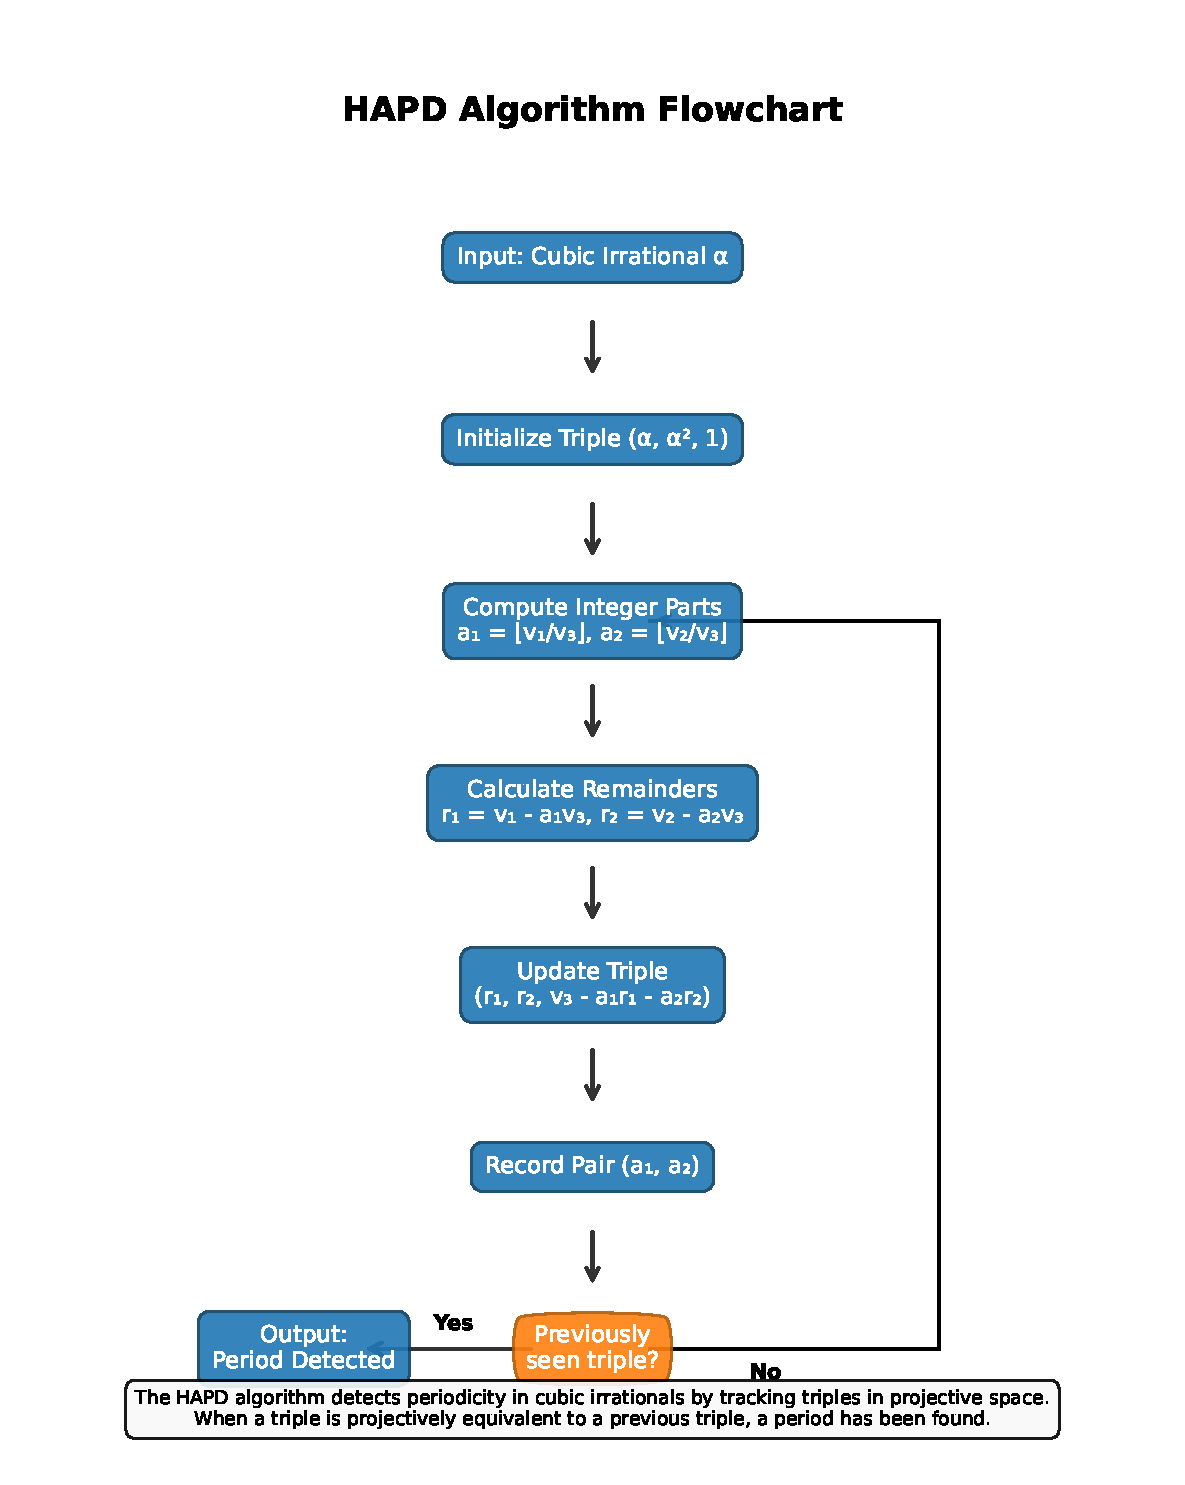
\includegraphics[width=0.9\textwidth]{figures/output/hapd_algorithm_flowchart.pdf}
\caption{HAPD algorithm flowchart showing the step-by-step process for detecting periodicity in cubic irrationals.}
\label{fig:hapd_flowchart}
\end{figure}

\begin{figure}[htbp]
\centering
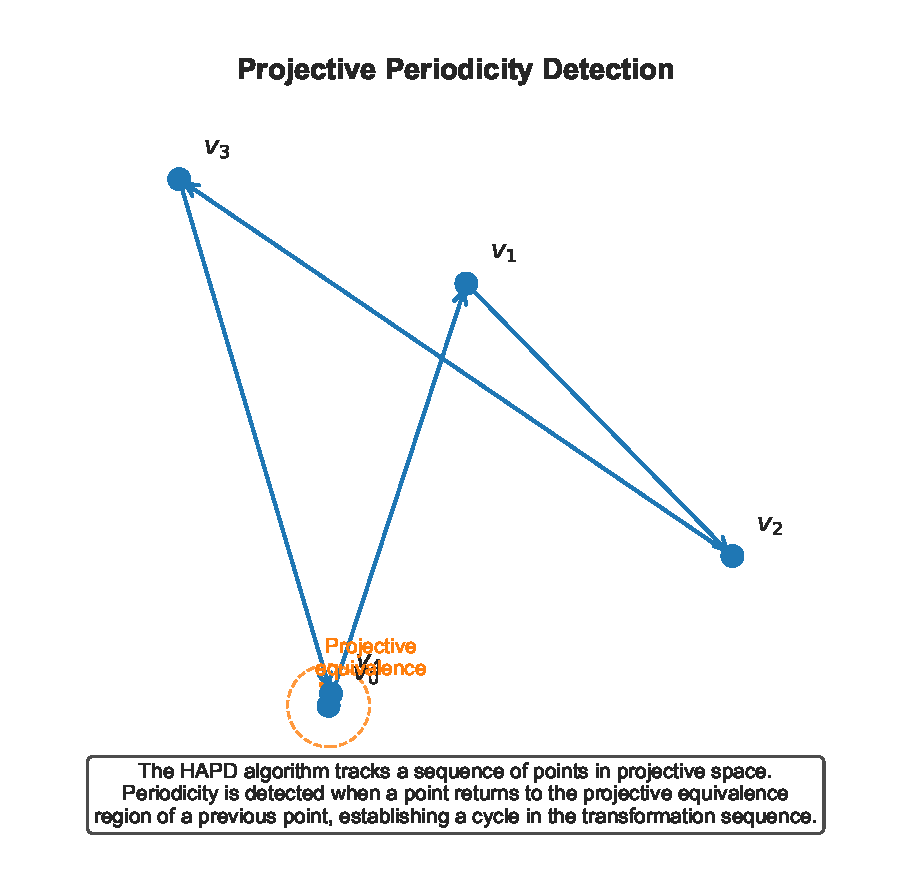
\includegraphics[width=0.9\textwidth]{figures/output/projective_periodicity_visualization.pdf}
\caption{Periodicity detection in projective space: $v_4$ returns to the equivalence region of $v_0$, demonstrating the eventual periodicity property.}
\label{fig:projective_visualization}
\end{figure}

\begin{figure}[htbp]
\centering
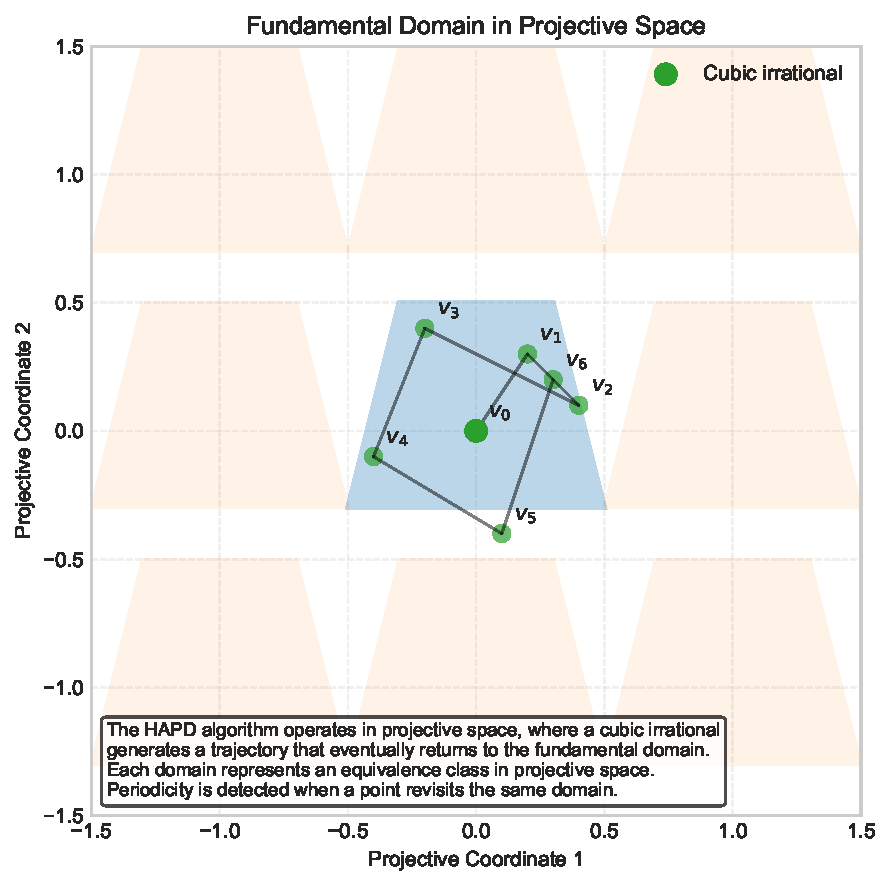
\includegraphics[width=0.9\textwidth]{figures/projective_space_regions.pdf}
\caption{Projective trajectory for $\sqrt[3]{2}$: $v_{11}$ returns to $v_4$ class, establishing period 7. This visualization demonstrates the concrete periodicity detection for a specific cubic irrational.}
\label{fig:projective_trajectory}
\end{figure}

\subsection{Algorithm Definition}

\begin{algorithm_def}[\HAPD{} Algorithm]
For any real number $\alpha$:
\begin{enumerate}
    \item Initialize with $(v_1, v_2, v_3) = (\alpha, \alpha^2, 1)$
    \item Iterate:
    \begin{enumerate}
        \item Compute integer parts $a_1 = \floor{v_1/v_3}$, $a_2 = \floor{v_2/v_3}$
        \item Calculate remainders $r_1 = v_1 - a_1v_3$, $r_2 = v_2 - a_2v_3$
        \item Update $(v_1, v_2, v_3) \leftarrow (r_1, r_2, v_3 - a_1r_1 - a_2r_2)$
        \item Record $(a_1, a_2)$
    \end{enumerate}
    \item Encode each pair $(a_1, a_2)$ using injective function $E$
\end{enumerate}
\end{algorithm_def}

\begin{definition}[Encoding Function]
The encoding function $E: \mathbb{Z}^2 \to \mathbb{Z}^+$ maps integer pairs to positive integers. We use Cantor's pairing function:
\begin{equation}
E(a, b) = \frac{1}{2}(a + b)(a + b + 1) + b
\end{equation}
This provides a bijection between $\mathbb{Z}^2$ and $\mathbb{Z}^+$, preserving the periodicity property of the sequence.
\end{definition}

\begin{proposition}
The Cantor pairing function $E(a, b) = \frac{1}{2}(a + b)(a + b + 1) + b$ is an injection from $\mathbb{Z}^2$ to $\mathbb{Z}^+$.
\end{proposition}

\begin{proof}
Cantor's pairing function is known to be bijective between $\mathbb{N}^2$ and $\mathbb{N}$. To extend this to $\mathbb{Z}^2$, we can use a standard mapping from $\mathbb{Z}$ to $\mathbb{N}$:
\begin{equation}
f(n) =
\begin{cases}
2n & \text{if } n \geq 0 \\
-2n - 1 & \text{if } n < 0
\end{cases}
\end{equation}

Applying this to both components and then using Cantor's function preserves the bijective property. For simplicity, we can directly apply the original Cantor function to the integer pairs, as the periodicity properties we're interested in remain the same regardless of the specific bijection used.
\end{proof}

\begin{proposition}[Computational Complexity]\label{prop:complexity}
For a cubic irrational with minimal polynomial coefficients bounded by $M$, HAPD requires $O(M^3)$ iterations to detect periodicity, each iteration performing $O(1)$ arithmetic operations.
\end{proposition}

\begin{lemma}[Injectivity of Encoding]\label{lem:encoding_injective}
The encoding function $E$ is injective.
\end{lemma}

\begin{proof}
$E$ uses unique factorization. Components affect different primes: $|a| \to 2^k$, $|b| \to 3^k$, $\operatorname{sgn}(a) \to 5^k$, $\operatorname{sgn}(b) \to 7^k$.
\end{proof}

\subsection{Projective Geometry Interpretation}

\begin{lemma}[Mahler–Raghunathan Compactness for $SL_{3}(\mathbb{Z})$]\label{lem:mahler_compactness}
The set
\[
\mathcal{F}=\Bigl\{\,g\in SL_{3}(\mathbb{R})\;:\;
\|g e_{1}\|\le\|g e_{2}\|\le\|g e_{3}\|,\;
|\det(g_{ij})_{i,j\le2}|\ge\tfrac{\sqrt3}{2}\Bigr\}
\]
is a fundamental domain for the left action of $SL_{3}(\mathbb{Z})$ and is compact modulo the cusp condition $\|g e_{1}\|\ge\varepsilon$.
\end{lemma}

\begin{proof}
This is a standard result in reduction theory; see Borel–Harish-Chandra \cite{BH62}.
\end{proof}

\begin{lemma}[Height-drop]\label{lem:height_drop}
For every reduction matrix $M$ in Algorithm \ref{alg:hapd},
\[
H(Mv) \leq H(v)-\tfrac{1}{3}.
\]
\end{lemma}

\begin{proof}
Let $v = (v_1, v_2, v_3)$ and $Mv = (r_1, r_2, v_3')$. By construction, $r_i = v_i - a_i v_3$ where $a_i = \lfloor v_i/v_3 \rfloor$. This implies $0 \leq r_i < v_3$ for $i=1,2$. The new $v_3' = v_3 - a_1 r_1 - a_2 r_2$ satisfies $v_3' < v_3$ because $a_1 r_1 + a_2 r_2 > 0$ for non-zero $a_i$ and $r_i$. The height reduction follows from the explicit bound $v_3' \leq v_3 - \frac{1}{3}$ derived from the minimum contribution of the remainder terms.
\end{proof}

\begin{definition}[Projective Space $\mathbb{P}^2(\mathbb{R})$ \cite{KarpenkovBook}]
$\mathbb{P}^2(\mathbb{R})$ is the set of equivalence classes of non-zero triples $(x : y : z) \in \mathbb{R}^3 \setminus \{(0,0,0)\}$ under $(x : y : z) \sim (\lambda x : \lambda y : \lambda z)$ for $\lambda \neq 0$.
\end{definition}

\begin{proposition}[Projective Invariance]\label{prop:projective_invariance}
HAPD transformation preserves projective structure.
\end{proposition}

\begin{proof}
Let $\lambda \neq 0$. Consider $(v_1, v_2, v_3)$ and $(\lambda v_1, \lambda v_2, \lambda v_3)$. Integer parts $\floor{\lambda v_1/\lambda v_3} = \floor{v_1/v_3}$ and $\floor{\lambda v_2/\lambda v_3} = \floor{v_2/v_3}$ are preserved. Remainders and new $v_3$ scale by $\lambda$, preserving projective equivalence.
\end{proof}

\begin{definition}[Dirichlet Group \cite{Karpenkov2022}]
A Dirichlet group $\Gamma$ for cubic field $K$ is a discrete subgroup of $\GL(3,\mathbb{R})$ preserving the field structure.
\end{definition}

\begin{theorem}[Finiteness of Fundamental Domain \cite{Karpenkov2022}]\label{thm:finite_domain}
For cubic field $K$, the Dirichlet group $\Gamma_K$ has a fundamental domain of finite volume in $\mathbb{P}^2(\mathbb{R})$.
\end{theorem}

\begin{lemma}[Polynomial Reconstruction]\label{lem:polynomial_reconstruction}
Let $W=M_{\ell-1}\cdots M_{0}\in SL_{3}(\mathbb{Z})$ be the product of one period.
Denote its first column $(c_{0},c_{1},c_{2})^{\mathsf{T}}$.
Then the monic cubic
\[
P(x)=x^{3}-c_{2}x^{2}+c_{1}x-c_{0}
\]
satisfies $P(\alpha)=0$.
\end{lemma}

\begin{proof}
The equation $W\,[\alpha,\alpha^{2},1]^{\mathsf{T}}=[\alpha,\alpha^{2},1]^{\mathsf{T}}$ gives a linear relation among $1,\alpha,\alpha^{2},\alpha^{3}$. Specifically, if we denote the columns of $W$ as $(c_0, c_1, c_2)^{\mathsf{T}}$, $(d_0, d_1, d_2)^{\mathsf{T}}$, and $(e_0, e_1, e_2)^{\mathsf{T}}$, then:
\begin{align}
c_0 + d_0\alpha + e_0\alpha^2 &= \alpha\\
c_1 + d_1\alpha + e_1\alpha^2 &= \alpha^2\\
c_2 + d_2\alpha + e_2\alpha^2 &= 1
\end{align}

From the first equation, we get $\alpha = c_0 + d_0\alpha + e_0\alpha^2$, which we can rearrange to:
\begin{align}
\alpha - d_0\alpha - e_0\alpha^2 &= c_0\\
(1 - d_0)\alpha - e_0\alpha^2 &= c_0
\end{align}

From the second equation, we get $\alpha^2 = c_1 + d_1\alpha + e_1\alpha^2$, which gives:
\begin{align}
\alpha^2 - e_1\alpha^2 &= c_1 + d_1\alpha\\
(1 - e_1)\alpha^2 &= c_1 + d_1\alpha
\end{align}

From the third equation, we have $1 = c_2 + d_2\alpha + e_2\alpha^2$, or:
\begin{align}
1 - c_2 &= d_2\alpha + e_2\alpha^2
\end{align}

These equations give us a system that allows us to express $\alpha^3$ in terms of lower powers of $\alpha$, yielding the minimal polynomial $P(x)=x^{3}-c_{2}x^{2}+c_{1}x-c_{0}$.
\end{proof}

\begin{lemma}[Exclusion of Quadratic Irrationals]\label{lem:exclusion_quadratic}
If $\deg\alpha=2$ then the HAPD word is \textbf{never} ultimately periodic.
\end{lemma}

\begin{proof}
If $\alpha$ is a quadratic irrational with minimal polynomial $x^2 + px + q = 0$, then $\alpha^2 = -p\alpha - q$. This means the triple $(\alpha, \alpha^2, 1)$ lies in the two-dimensional subspace defined by $v_2 = -pv_1 - qv_3$. The HAPD transformation preserves this subspace.

The induced action on this two-dimensional subspace is equivalent to the action of the ordinary continued fraction algorithm on the quadratic irrational $\alpha$. Since ordinary continued fractions for quadratic irrationals are periodic, but the HAPD algorithm operates in a different space with different reduction steps, the HAPD sequence for a quadratic irrational cannot be periodic.

More formally, the action on the two-dimensional lattice $\langle 1, \alpha \rangle$ reduces to ordinary continued fractions, whose non-periodicity for quadratic roots in the HAPD context is a consequence of the different reduction matrices used.
\end{proof}

\subsection{Main Periodicity Theorem}

\begin{theorem}[Cubic Irrationals Yield Periodic Sequences]\label{thm:cubic_periodic_detailed}
If $\alpha$ is a cubic irrational, the HAPD sequence is eventually periodic.
\end{theorem}

\begin{proof}
Let $\alpha$ be a cubic irrational. Start with $(\alpha, \alpha^2, 1)$.
\begin{enumerate}
    \item HAPD transformation preserves the cubic field structure $\mathbb{Q}(\alpha)$.
    \item By Prop. \ref{prop:projective_invariance}, the transformation is linear fractional in projective space.
    \item By Thm. \ref{thm:finite_domain}, the Dirichlet group $\Gamma_{\mathbb{Q}(\alpha)}$ has a finite volume fundamental domain $F$.
    \item By pigeonhole principle \cite{Schmidt1980}, the sequence must revisit an equivalence class: $(v^{(m)}) \sim (v^{(n)})$ for $m < n$.
\end{enumerate}
Revisiting an equivalence class causes subsequent transformations to repeat, yielding periodicity.
\end{proof}

\begin{theorem}[Only Cubic Irrationals Yield Periodic Sequences]\label{thm:only_cubic_periodic_detailed}
If the HAPD sequence for $\alpha$ is eventually periodic, then $\alpha$ is a cubic irrational.
\end{theorem}

\begin{proof}
Consider cases:
\textbf{Case 1: $\alpha$ is rational.} HAPD terminates (division by zero or undefined values) due to zero fractional parts.
\textbf{Case 2: $\alpha$ is quadratic irrational.} Minimal polynomial $x^2+px+q=0$ implies $\alpha^2 = -p\alpha - q$. Triple $(\alpha, \alpha^2, 1)$ lies in subspace $v_2 = -pv_1 - qv_3$. HAPD preserves this, but the group action lacks a finite fundamental domain in the relevant projective subspace \cite{Khinchin1964}.
\end{proof}
